\documentclass[margin=1em]{standalone}

\usepackage{pgfplots}
\pgfplotsset{compat=1.10}   % in my packages used compat=1.15
\usepgfplotslibrary{fillbetween}
\usepackage{pgf}
\usepackage{tikz}
\usetikzlibrary{patterns,arrows, arrows.meta,calc,decorations.pathmorphing,backgrounds, positioning,fit,petri,decorations.fractals}
\usetikzlibrary{matrix}

\usepackage[table,dvipsnames]{tudscrcolor}

\usepackage[default]{opensans}

\begin{document}
	\color{cddarkblue}
	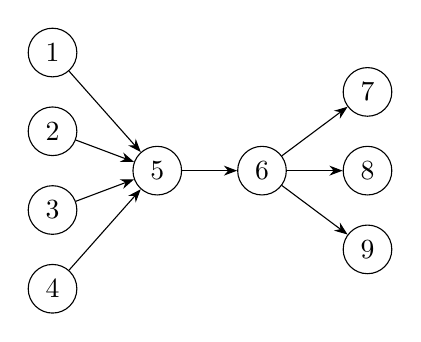
\begin{tikzpicture}		
		\node [circle,draw] (1) at (0,1.5)  {$1$};
		\node [circle,draw] (2) at (0,0.5)  {$2$};
		\node [circle,draw] (3) at (0,-0.5) {$3$};
		\node [circle,draw] (4) at (0,-1.5) {$4$};
		
		\node [circle,draw] (5) at (1.33,0)  {$5$};
		\node [circle,draw] (6) at (2.66,0)  {$6$};
		
		\node [circle,draw] (7) at (4,1)  {$7$};
		\node [circle,draw] (8) at (4,0)  {$8$};
		\node [circle,draw] (9) at (4,-1) {$9$};
		
		% Kanten
		% \path (1) -> node[weight] {$3$} (3)
		\draw[->, arrows=-Stealth] (1) -> (5);
		\draw[->, arrows=-Stealth] (2) -> (5);
		\draw[->, arrows=-Stealth] (3) -> (5);
		\draw[->, arrows=-Stealth] (4) -> (5);
		\draw[->, arrows=-Stealth] (5) -> (6);
		\draw[->, arrows=-Stealth] (6) -> (7);
		\draw[->, arrows=-Stealth] (6) -> (8);
		\draw[->, arrows=-Stealth] (6) -> (9);
	\end{tikzpicture}
\end{document}